% =============================================================================
% Neural Receiver System Architecture for OAM-FSO
% Standalone LaTeX — compile with: pdflatex system_architecture.tex
% Or use \input{} in main manuscript
% =============================================================================
\documentclass[lettersize,journal]{IEEEtran}
\usepackage{amsmath,amsfonts,amssymb}
\usepackage{tikz}
\usetikzlibrary{arrows.meta,positioning,shapes.geometric,fit,backgrounds}

\begin{document}

%------------------------------------------------------------------------------
% Figure 1: Neural Receiver Inference Architecture
%------------------------------------------------------------------------------
\begin{figure}[!t]
\centering
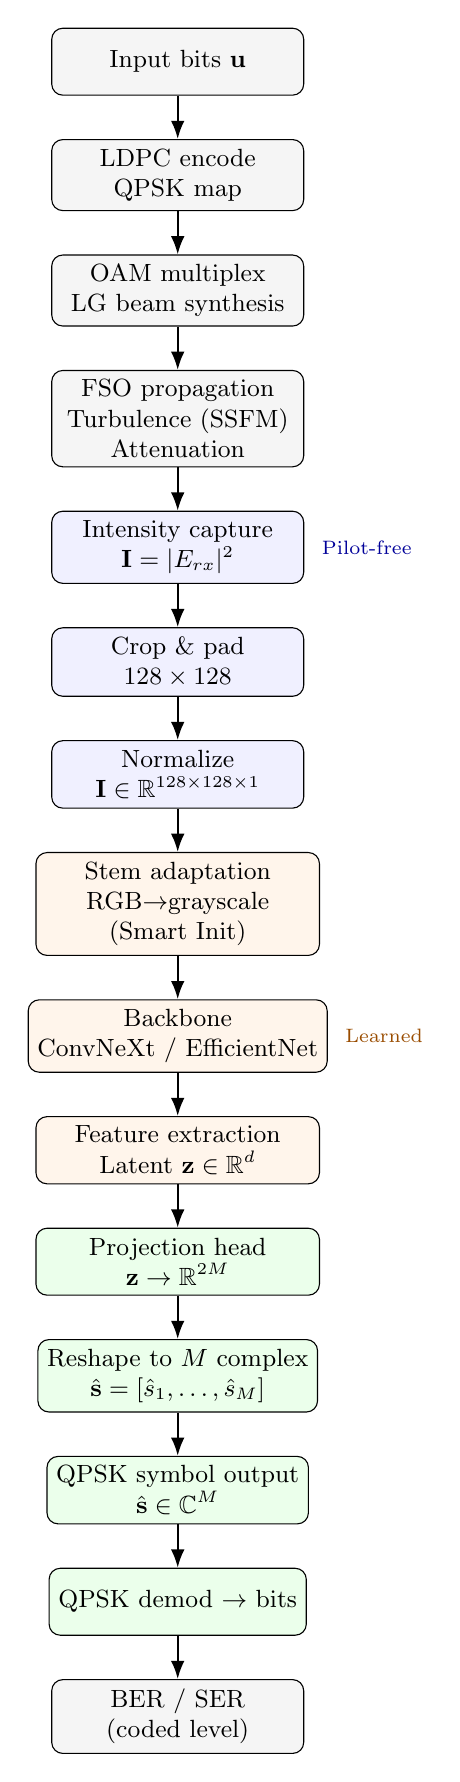
\begin{tikzpicture}[
  node distance=5.5mm,
  block/.style={
    draw,
    rounded corners,
    align=center,
    minimum width=3.2cm,
    minimum height=0.85cm,
    font=\small
  },
  wideblock/.style={
    draw,
    rounded corners,
    align=center,
    minimum width=3.6cm,
    minimum height=0.85cm,
    font=\small
  },
  layer/.style={
    draw,
    rounded corners,
    dashed,
    inner sep=4pt,
    fit=#1
  },
  line/.style={-Latex, thick}
]

% --- Shared TX/Channel (same as baseline, abbreviated) ---
\node[block,fill=gray!8] (tx_bits) {Input bits $\mathbf{u}$};

\node[block,below=of tx_bits,fill=gray!8] (tx_enc)
{LDPC encode\\QPSK map};

\node[block,below=of tx_enc,fill=gray!8] (tx_oam)
{OAM multiplex\\LG beam synthesis};

\node[block,below=of tx_oam,fill=gray!8] (channel)
{FSO propagation\\Turbulence (SSFM)\\Attenuation};

% --- Neural branch: intensity capture (divergence from classical) ---
\node[block,below=of channel,fill=blue!6] (intensity)
{Intensity capture\\$\mathbf{I} = |E_{rx}|^2$};

\node[block,below=of intensity,fill=blue!6] (crop)
{Crop \& pad\\$128 \times 128$};

\node[block,below=of crop,fill=blue!6] (norm)
{Normalize\\$\mathbf{I} \in \mathbb{R}^{128\times128\times1}$};

% --- Neural backbone ---
\node[wideblock,below=of norm,fill=orange!8] (stem)
{Stem adaptation\\RGB$\to$grayscale\\(Smart Init)};

\node[wideblock,below=of stem,fill=orange!8] (backbone)
{Backbone\\ConvNeXt / EfficientNet};

\node[wideblock,below=of backbone,fill=orange!8] (features)
{Feature extraction\\Latent $\mathbf{z} \in \mathbb{R}^d$};

% --- Symbol regression head ---
\node[wideblock,below=of features,fill=green!8] (head)
{Projection head\\$\mathbf{z} \to \mathbb{R}^{2M}$};

\node[block,below=of head,fill=green!8] (reshape)
{Reshape to $M$ complex\\$\hat{\mathbf{s}} = [\hat{s}_1,\ldots,\hat{s}_M]$};

\node[block,below=of reshape,fill=green!8] (out)
{QPSK symbol output\\$\hat{\mathbf{s}} \in \mathbb{C}^M$};

% Coded-level BER (no LDPC decode in current implementation)
\node[block,below=of out,fill=green!8] (demod)
{QPSK demod $\to$ bits};

\node[block,below=of demod,fill=gray!8] (ber)
{BER / SER\\(coded level)};

% Arrows
\draw[line] (tx_bits) -- (tx_enc);
\draw[line] (tx_enc) -- (tx_oam);
\draw[line] (tx_oam) -- (channel);
\draw[line] (channel) -- (intensity);
\draw[line] (intensity) -- (crop);
\draw[line] (crop) -- (norm);
\draw[line] (norm) -- (stem);
\draw[line] (stem) -- (backbone);
\draw[line] (backbone) -- (features);
\draw[line] (features) -- (head);
\draw[line] (head) -- (reshape);
\draw[line] (reshape) -- (out);
\draw[line] (out) -- (demod);
\draw[line] (demod) -- (ber);

% Layer labels (optional, can comment out for cleaner look)
\node[font=\scriptsize,right=1mm of intensity,text=blue!60!black] {Pilot-free};
\node[font=\scriptsize,right=1mm of backbone,text=orange!60!black] {Learned};

\end{tikzpicture}
\label{fig:neural_inference}
\end{figure}

\clearpage

%------------------------------------------------------------------------------
% Figure 2: Training Pipeline (Curriculum Learning)
%------------------------------------------------------------------------------
\begin{figure}[!t]
\centering
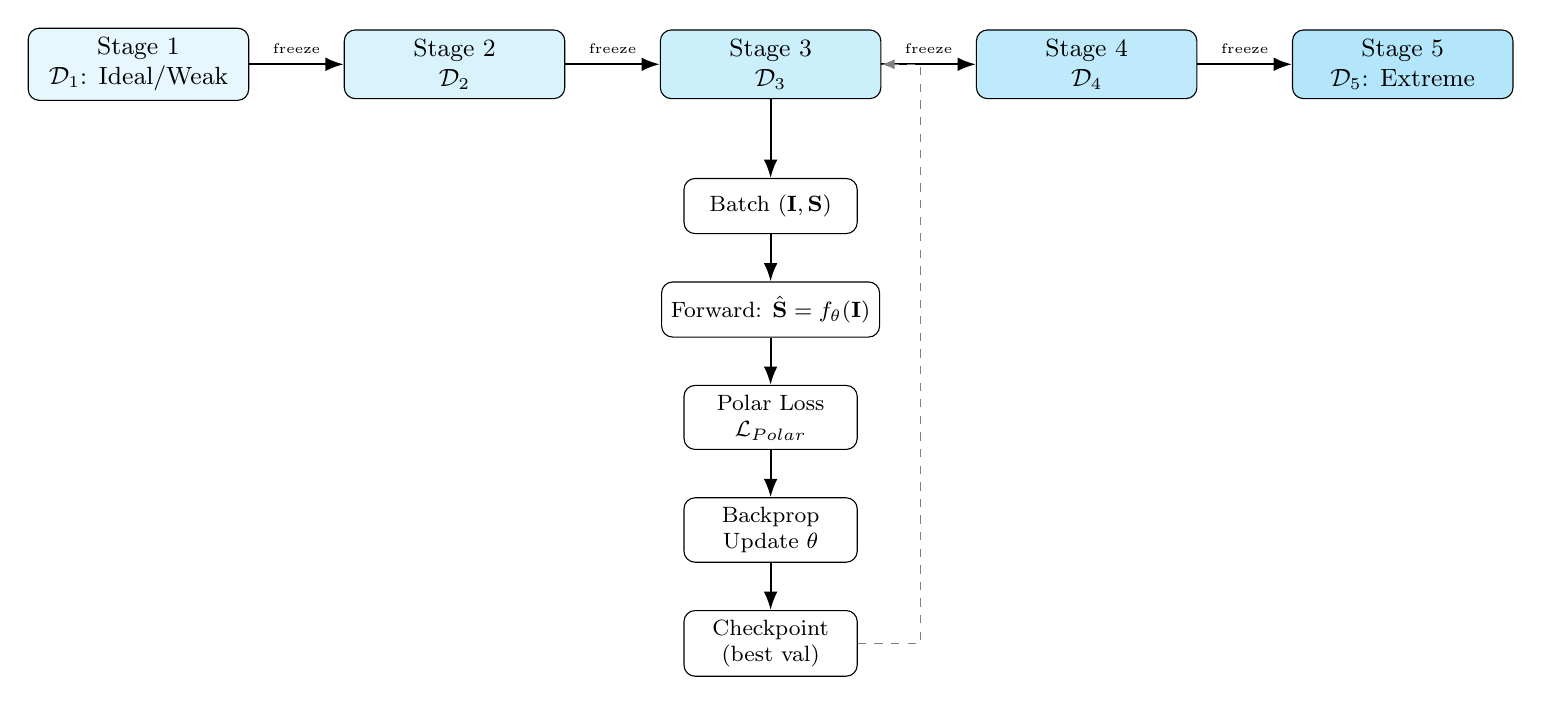
\begin{tikzpicture}[
  node distance=6mm,
  block/.style={
    draw,
    rounded corners,
    align=center,
    minimum width=2.8cm,
    minimum height=0.8cm,
    font=\small
  },
  datablock/.style={
    draw,
    rounded corners,
    align=center,
    minimum width=2.2cm,
    minimum height=0.7cm,
    font=\footnotesize
  },
  line/.style={-Latex, thick},
  dline/.style={-Latex, dashed, gray}
]

% Curriculum stages
\node[block,fill=cyan!10] (stage1) {Stage 1\\$\mathcal{D}_1$: Ideal/Weak};

\node[block,right=12mm of stage1,fill=cyan!15] (stage2) {Stage 2\\$\mathcal{D}_2$};

\node[block,right=12mm of stage2,fill=cyan!20] (stage3) {Stage 3\\$\mathcal{D}_3$};

\node[block,right=12mm of stage3,fill=cyan!25] (stage4) {Stage 4\\$\mathcal{D}_4$};

\node[block,right=12mm of stage4,fill=cyan!30] (stage5) {Stage 5\\$\mathcal{D}_5$: Extreme};

% Per-stage flow
\node[datablock,below=10mm of stage3] (batch) {Batch $(\mathbf{I},\mathbf{S})$};

\node[datablock,below=of batch] (forward) {Forward: $\hat{\mathbf{S}}=f_\theta(\mathbf{I})$};

\node[datablock,below=of forward] (loss) {Polar Loss\\$\mathcal{L}_{Polar}$};

\node[datablock,below=of loss] (backprop) {Backprop\\Update $\theta$};

\node[datablock,below=of backprop] (ckpt) {Checkpoint\\(best val)};

% Curriculum arrows (stage transfer)
\draw[line] (stage1) -- node[above,font=\tiny] {freeze} (stage2);
\draw[line] (stage2) -- node[above,font=\tiny] {freeze} (stage3);
\draw[line] (stage3) -- node[above,font=\tiny] {freeze} (stage4);
\draw[line] (stage4) -- node[above,font=\tiny] {freeze} (stage5);

% Per-stage loop
\draw[line] (stage3.south) -- ++(0,-3mm) -| (batch.north);
\draw[line] (batch) -- (forward);
\draw[line] (forward) -- (loss);
\draw[line] (loss) -- (backprop);
\draw[line] (backprop) -- (ckpt);
\draw[dline] (ckpt.east) -- ++(8mm,0) |- (stage3.east);

\end{tikzpicture}
\label{fig:neural_training}
\end{figure}

\clearpage

%------------------------------------------------------------------------------
% Figure 3: Combined High-Level Comparison (Classical vs Neural)
%------------------------------------------------------------------------------
\begin{figure}[!t]
\centering
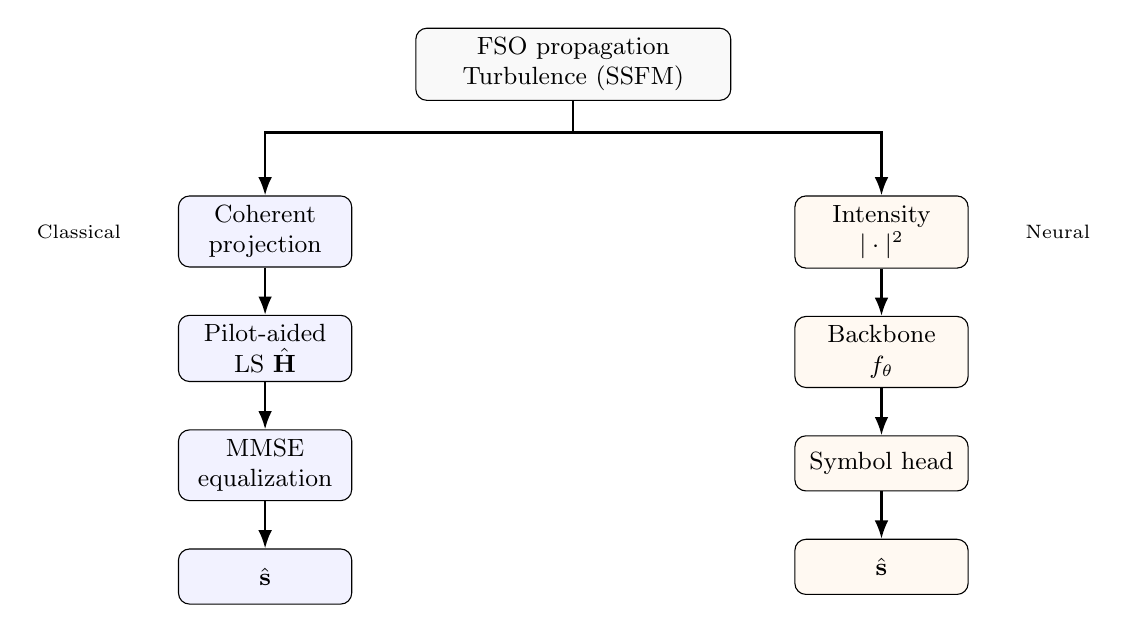
\begin{tikzpicture}[
  node distance=6mm,
  block/.style={
    draw,
    rounded corners,
    align=center,
    minimum height=0.7cm,
    font=\small
  },
  line/.style={-Latex, thick}
]

% Shared channel
\node[block,minimum width=4cm,fill=gray!5] (channel) {FSO propagation\\Turbulence (SSFM)};

% Classical branch
\node[block,below left=12mm and 8mm of channel,fill=blue!5,minimum width=2.2cm] (class_proj)
{Coherent\\projection};

\node[block,below=of class_proj,fill=blue!5,minimum width=2.2cm] (class_est)
{Pilot-aided\\LS $\hat{\mathbf{H}}$};

\node[block,below=of class_est,fill=blue!5,minimum width=2.2cm] (class_eq)
{MMSE\\equalization};

\node[block,below=of class_eq,fill=blue!5,minimum width=2.2cm] (class_out)
{$\hat{\mathbf{s}}$};

% Neural branch
\node[block,below right=12mm and 8mm of channel,fill=orange!5,minimum width=2.2cm] (neural_int)
{Intensity\\$|\cdot|^2$};

\node[block,below=of neural_int,fill=orange!5,minimum width=2.2cm] (neural_bb)
{Backbone\\$f_\theta$};

\node[block,below=of neural_bb,fill=orange!5,minimum width=2.2cm] (neural_head)
{Symbol head};

\node[block,below=of neural_head,fill=orange!5,minimum width=2.2cm] (neural_out)
{$\hat{\mathbf{s}}$};

% Arrows from channel
\draw[line] (channel.south) -- ++(0,-4mm) -| (class_proj.north);
\draw[line] (channel.south) -- ++(0,-4mm) -| (neural_int.north);

\draw[line] (class_proj) -- (class_est);
\draw[line] (class_est) -- (class_eq);
\draw[line] (class_eq) -- (class_out);

\draw[line] (neural_int) -- (neural_bb);
\draw[line] (neural_bb) -- (neural_head);
\draw[line] (neural_head) -- (neural_out);

% Labels (positioned outward to avoid overlap with branch arrows)
\node[left=6mm of class_proj,font=\scriptsize,anchor=east] {Classical};
\node[right=6mm of neural_int,font=\scriptsize,anchor=west] {Neural};

\end{tikzpicture}
\label{fig:neural_vs_classical}
\end{figure}

\end{document}
